\section{\uppercase{Results}}\label{sec:results}

\noindent Results text.

Active perception environment - 1 sensor

\begin{figure}
	\centering
	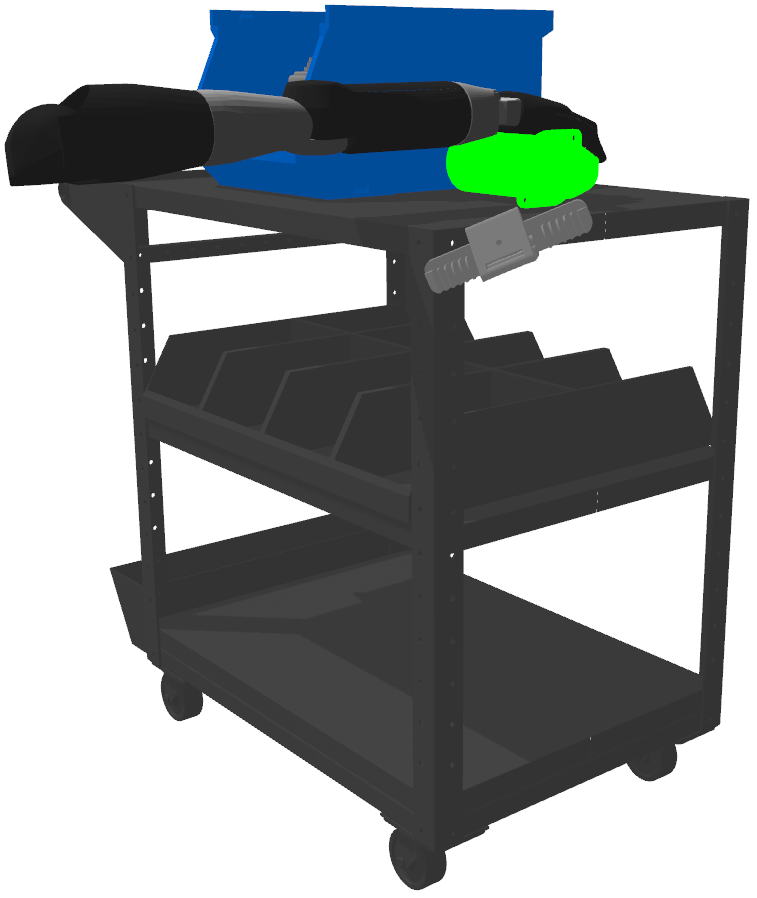
\includegraphics[height=.2\textwidth]{best-views-estimation/active-perception/1-sensor/gazebo-corner}\hspace{4em}
	\includegraphics[height=.2\textwidth]{best-views-estimation/active-perception/1-sensor/rviz-front-corner}\\
	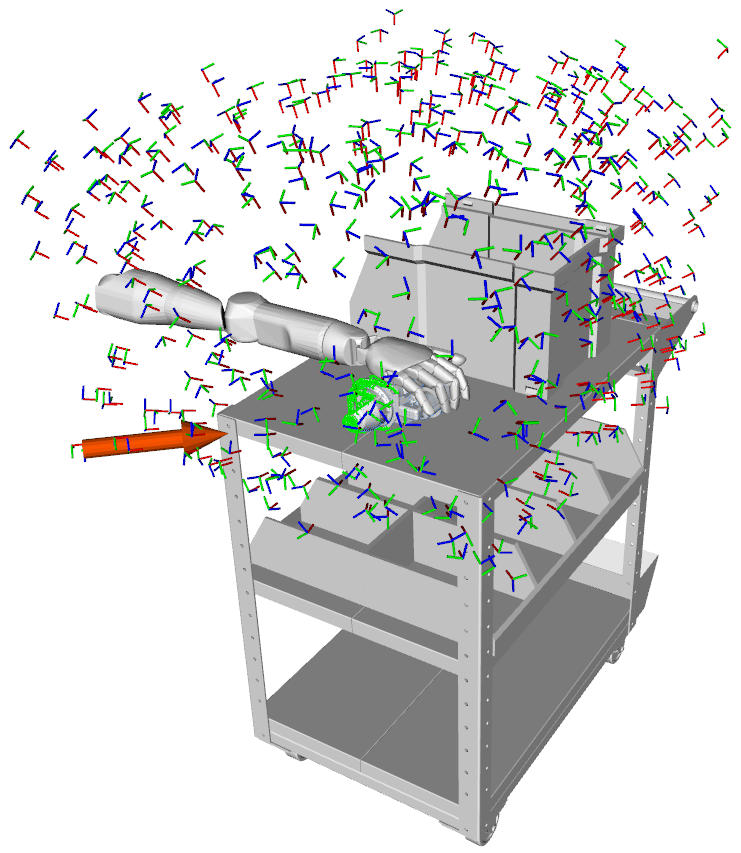
\includegraphics[height=.2\textwidth]{best-views-estimation/active-perception/1-sensor/rviz-back-corner}\hspace{2em}
	\includegraphics[height=.2\textwidth]{best-views-estimation/active-perception/1-sensor/rviz-top}
	\caption{Estimation of the best sensor position for the active perception environment with a 27.73\% of surface area coverage (top left showing the Gazebo color rendering and remaining images displaying the best sensor as a large red arrow, the deployed sensors as small coordinate frames and the observed sensor data as green spheres)}
\end{figure}


Active perception environment - 3 sensors

\begin{figure}
	\centering
	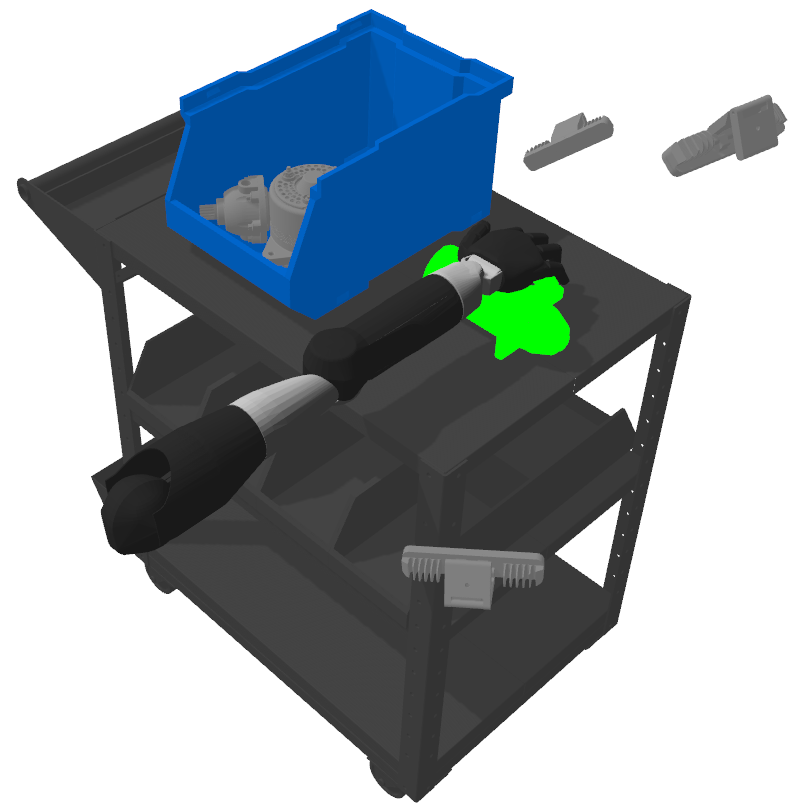
\includegraphics[height=.2\textwidth]{best-views-estimation/active-perception/3-sensors/gazebo-front-right-corner}\hspace{4em}
	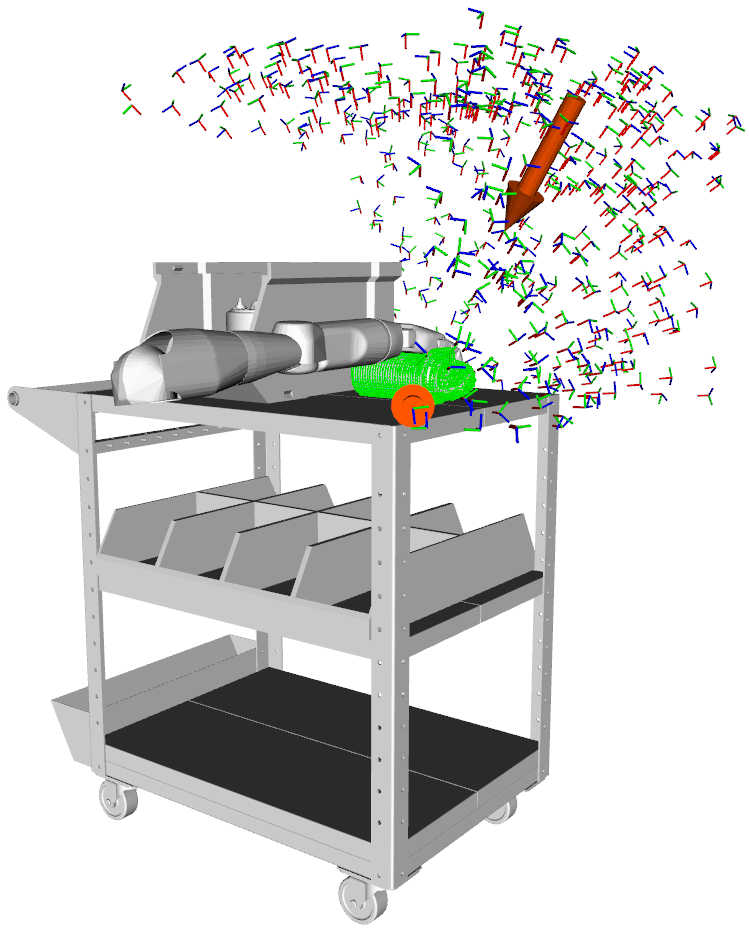
\includegraphics[height=.2\textwidth]{best-views-estimation/active-perception/3-sensors/rviz-front-right}\\
	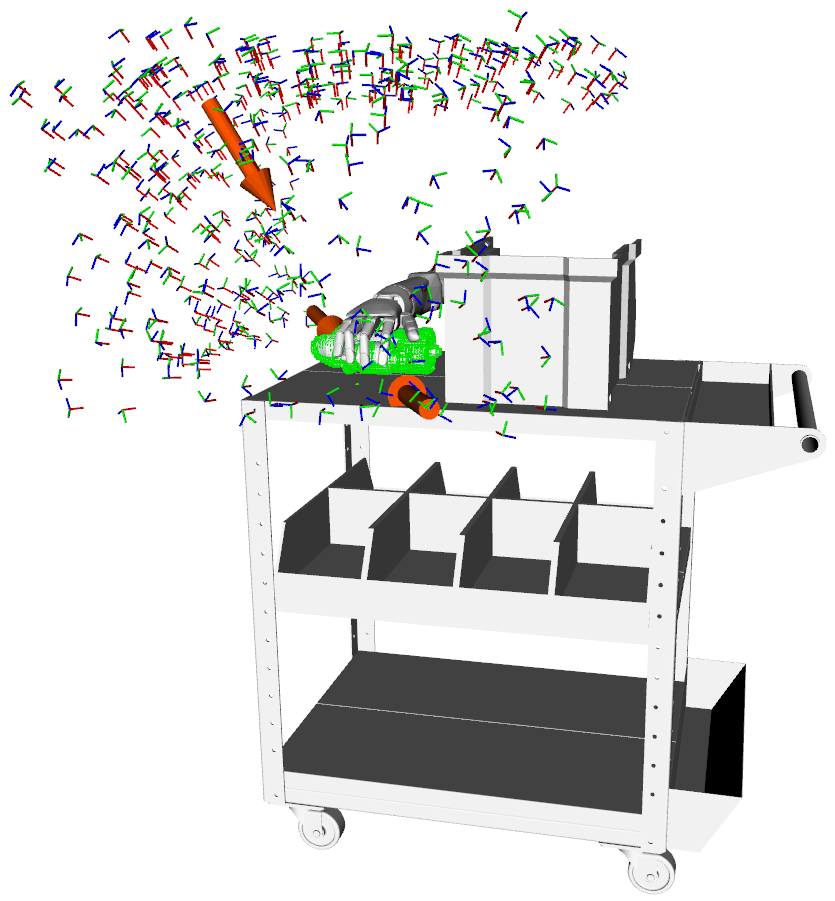
\includegraphics[height=.2\textwidth]{best-views-estimation/active-perception/3-sensors/rviz-back-left}\hspace{2em}
	\includegraphics[height=.2\textwidth]{best-views-estimation/active-perception/3-sensors/rviz-top}
	\caption{Estimation of the 3 best sensors disposition for the active perception environment with a 61.91\% of surface area coverage}
\end{figure}


Bin picking environment - 1 sensor

\begin{figure}
	\centering
	\includegraphics[height=.14\textwidth]{best-views-estimation/bin-picking/1-sensor/gazebo-top}\hspace{2em}
	\includegraphics[height=.14\textwidth]{best-views-estimation/bin-picking/1-sensor/rviz-front}\\
	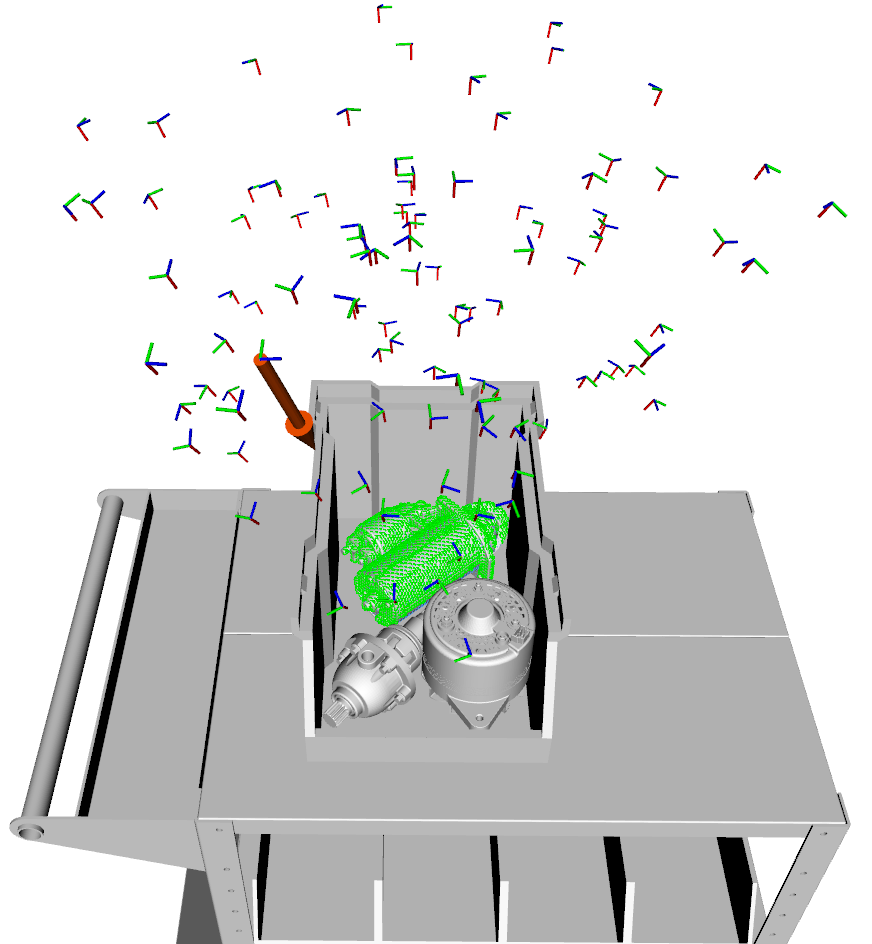
\includegraphics[height=.2\textwidth]{best-views-estimation/bin-picking/1-sensor/rviz-top-front}\hspace{2em}
	\includegraphics[height=.2\textwidth]{best-views-estimation/bin-picking/1-sensor/rviz-top}
	\caption{Estimation of the best sensor position for the bin picking environment with a 45.10\% of surface area coverage}
\end{figure}


Bin picking environment - 5 sensors

\begin{figure}
	\centering
	\includegraphics[height=.19\textwidth]{best-views-estimation/bin-picking/5-sensors/gazebo-front}\hspace{2em}
	\includegraphics[height=.14\textwidth]{best-views-estimation/bin-picking/5-sensors/rviz-top}\\
	\includegraphics[height=.2\textwidth]{best-views-estimation/bin-picking/5-sensors/rviz-corner}\hspace{2em}
	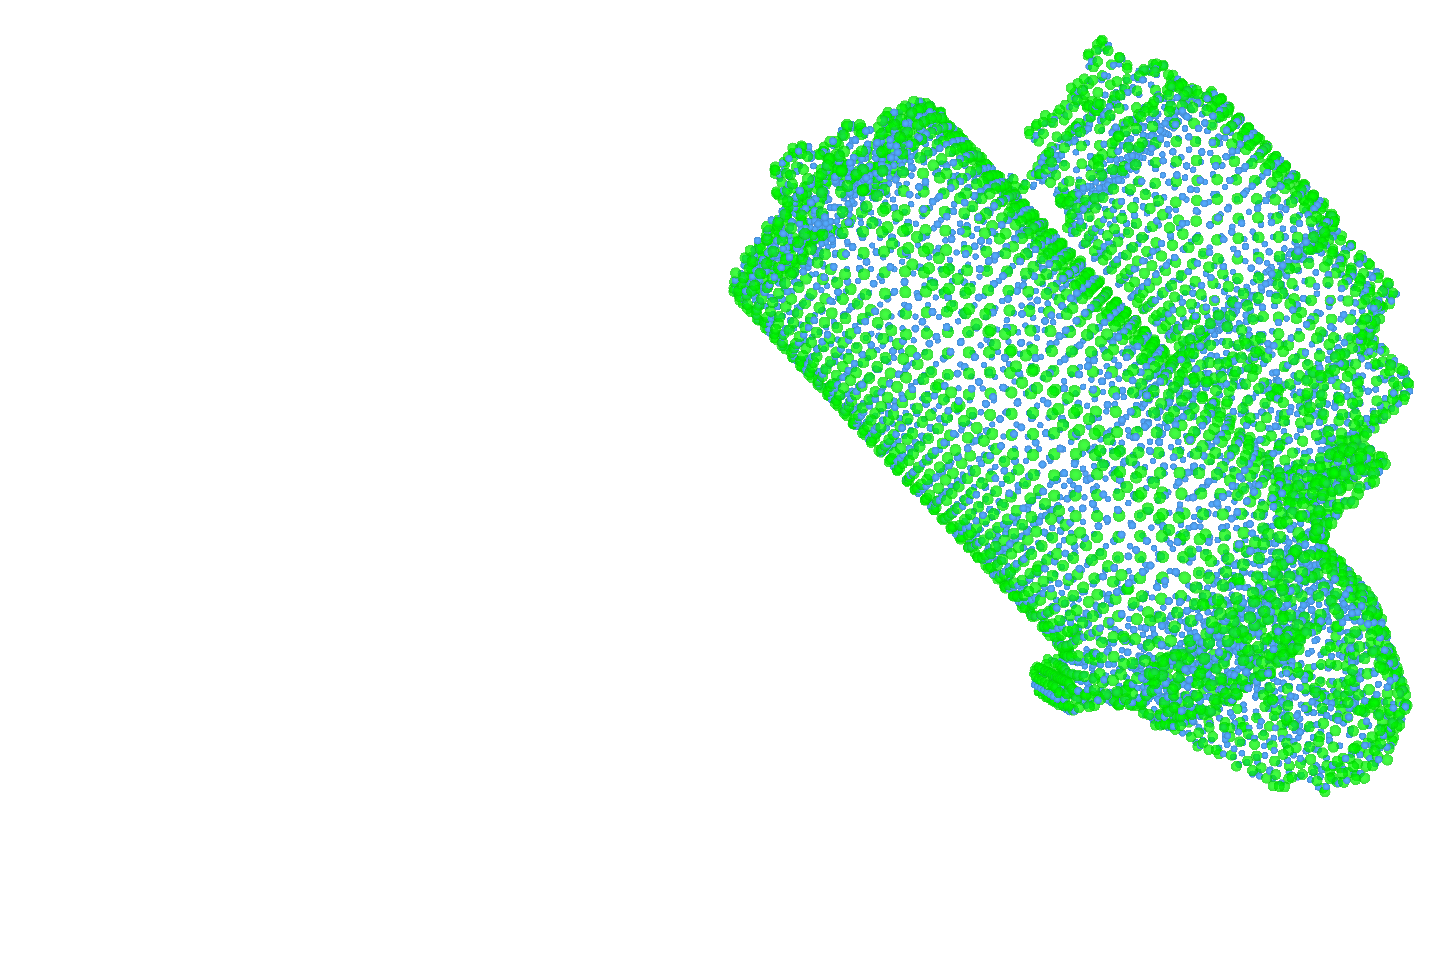
\includegraphics[height=.14\textwidth]{best-views-estimation/bin-picking/5-sensors/rviz-sensor-data}
	\caption{Estimation of the 5 best sensors disposition for the bin picking environment with a 64.63\% of surface area coverage}
\end{figure}


Bin picking with occlusions environment - 1 sensor

\begin{figure}
	\centering
	\includegraphics[height=.13\textwidth]{best-views-estimation/bin-picking-with-occlusions/1-sensor/gazebo-top}\hspace{2em}
	\includegraphics[height=.13\textwidth]{best-views-estimation/bin-picking-with-occlusions/1-sensor/rviz-corner}\\
	\includegraphics[height=.2\textwidth]{best-views-estimation/bin-picking-with-occlusions/1-sensor/rviz-front}\hspace{2em}
	\includegraphics[height=.2\textwidth]{best-views-estimation/bin-picking-with-occlusions/1-sensor/rviz-top}
	\caption{Estimation of the best sensor position for the bin picking with occlusions environment with a 19.27\% of surface area coverage}
\end{figure}


Bin picking with occlusions environment - 3 sensors

\begin{figure}
	\centering
	\includegraphics[height=.18\textwidth]{best-views-estimation/bin-picking-with-occlusions/3-sensors/gazebo-top}\hspace{2em}
	\includegraphics[height=.2\textwidth]{best-views-estimation/bin-picking-with-occlusions/3-sensors/rviz-front}\\
	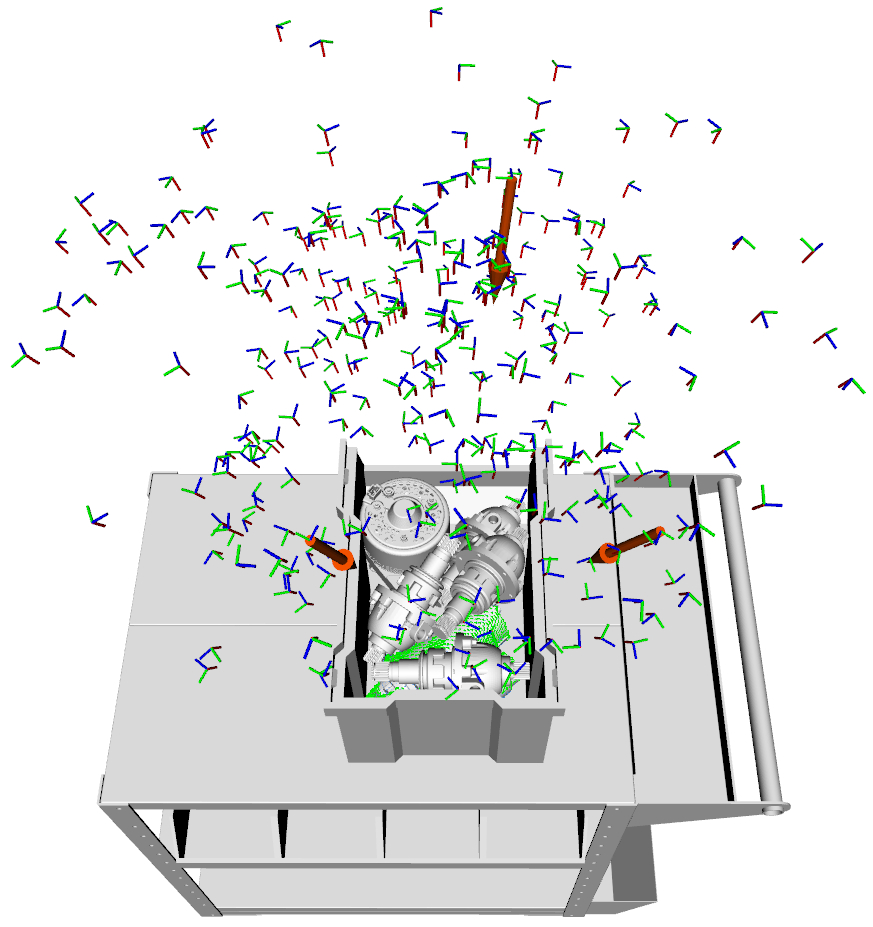
\includegraphics[height=.21\textwidth]{best-views-estimation/bin-picking-with-occlusions/3-sensors/rviz-top-back}\hspace{2em}
	\includegraphics[height=.21\textwidth]{best-views-estimation/bin-picking-with-occlusions/3-sensors/rviz-top}
	\caption{Estimation of the 3 best sensors disposition for the bin picking with occlusions environment with a 31.19\% of surface area coverage}
\end{figure}


Multiple bin picking with occlusions environment - 10 sensors

\begin{figure}
	\centering
	\includegraphics[height=.15\textwidth]{best-views-estimation/multiple-bin-picking-with-occlusions/10-sensors/gazebo-front}\hspace{2em}
	\includegraphics[height=.15\textwidth]{best-views-estimation/multiple-bin-picking-with-occlusions/10-sensors/rviz-front-corner}\\
	\includegraphics[height=.15\textwidth]{best-views-estimation/multiple-bin-picking-with-occlusions/10-sensors/rviz-front}\hspace{1.5em}
	\includegraphics[height=.15\textwidth]{best-views-estimation/multiple-bin-picking-with-occlusions/10-sensors/rviz-top}
	\caption{Estimation of the 10 best sensors disposition for the multiple bin picking with occlusions environment with a 43.93\% of surface area coverage}
\end{figure}
